\subsection{CultureID: Internet of Things, Robotics, Big Data, AI in Culture}

\noindent Context: Project co-financed by EU and Greek National Funds, under the call RESEARCH - CREATE -INNOVATE (project code: T2EDK-02000)\\
\noindent Aristotle University of Thessaloniki, Greece\\
\noindent Duration: 09/2020--09/2023\\

\noindent \textbf{In a nutshell}\\
\noindent \href{https://cultureid.web.auth.gr/?page_id=216&lang=en}{\texttt{[Website]}} \href{https://www.facebook.com/cultureID.Auth}{\texttt{[fb]}} \href{https://www.youtube.com/@cultureidproject}{\texttt{[Videos]}} \href{https://cultureid.web.auth.gr/?page_id=490}{\texttt{[Publications]}} \href{https://github.com/cultureid-auth-ros-packages}{\texttt{[Public code]}}\\


\begin{figure}[H]\centering
  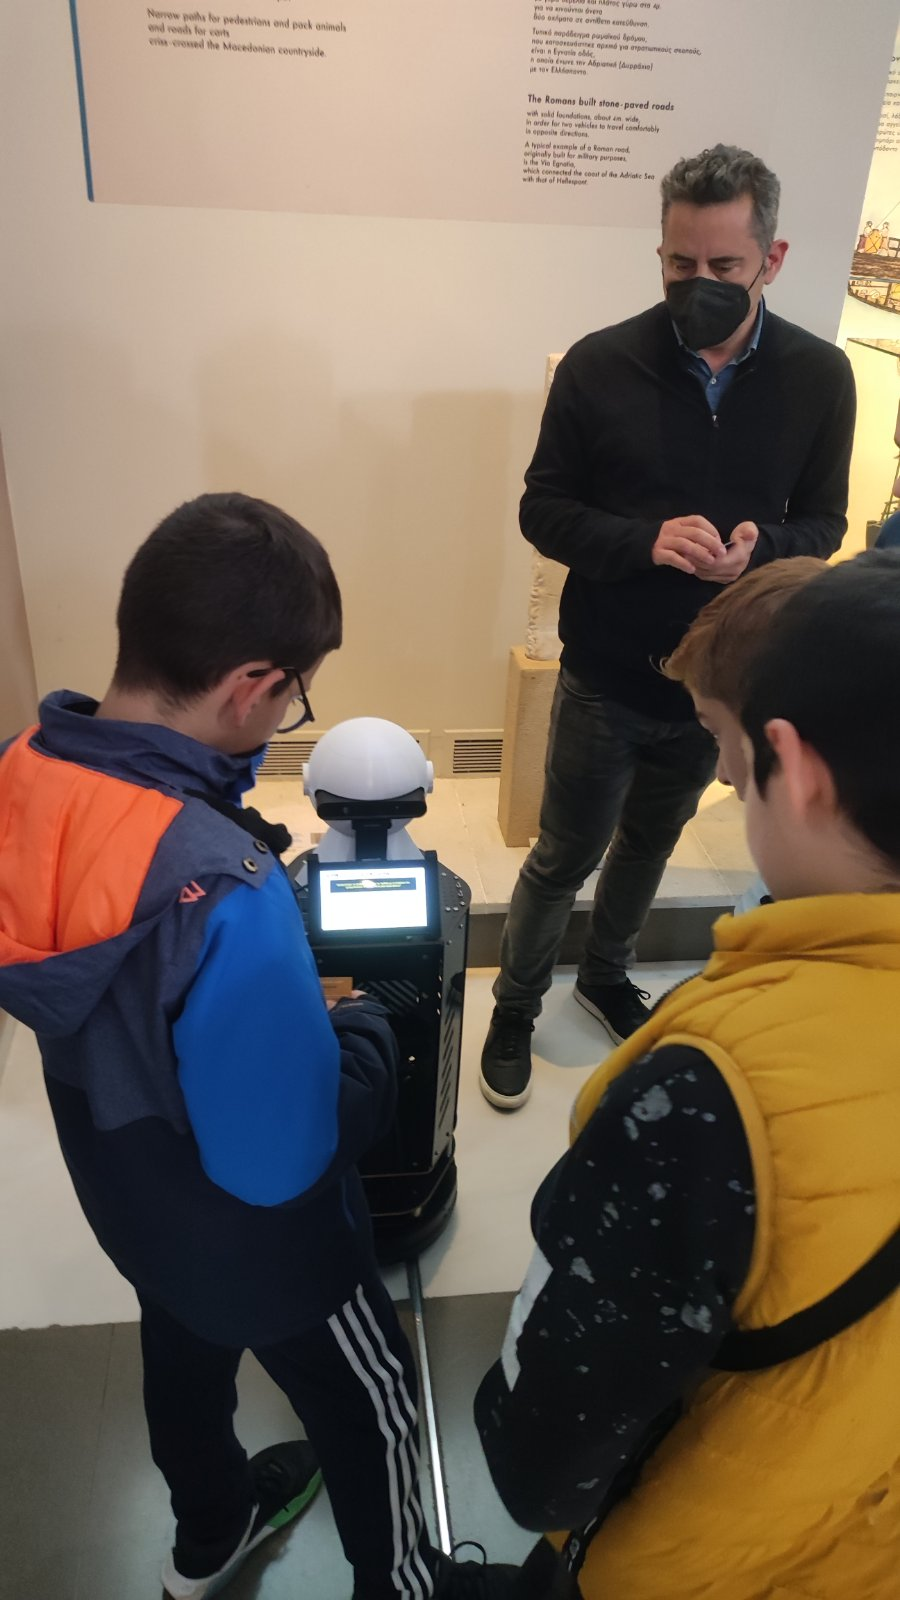
\includegraphics[scale=0.2]{images/cultureid/indy_at_museum.jpg}
  \caption{\small CultureID's robot acting as a game master with pupils from
           the 4th public elementary school of Thessaloniki}
  \label{fig:cultureid_indy}
\end{figure}

Among other things the project developed a social robot---Indy!---with the
explicit intent of bridging cultural facts, artefacts, works of art, and
general knowledge---over to the audience of a museum: in particular that of the
Archaeological Museum of Thessaloniki (AMTh), Greece. Specifically, I, in
partnership with the project's partners and our team's members, thought,
designed, implemented, deployed, and refined the systems concerning the two
activities that the robot was tasked to hold in the museum: (a) playing games
while acting as the game master with students whose school pays visit to the
museum, and (b) acting as a tour guide for specific displayed artefacts.


\subsubsection{Playing games with pupils}

The actual contents of the games, regardless of the nature of the game master
were expertly crafted by Dr (of Education) Sofia Pliasa. The games focused
around AMTh's exhibitions and themes of artefacts, e.g. armament, daily habits,
grooming (καλλωπισμός), hunting, and others. Indy, with a clear mind of the
pupils' abilities (ages ranged from 8 to 14), organised them into groups, asked
them questions with regard to themes and artefacts around them, gave them hints
and instructions--all while handling groups in a round-robin fashion.

The interaction between the robot and the pupils was performed via a screen,
placed at an appropriate-for-the-children height on the robot, speakers, and a
panoramic microphone array. RFID technology was used in order to engage the
pupils and arouse their sense of playing and therefore alleviating their
boredom, prevalent in the era before Indy. These are all summarised in the two
images that follow.

---Of course, one would ask: ``Alexandros, what is the use of a robot for
playing this type of game you are describing when an static computer could
perform the same task?" The first difference is that the robot cheered on
groups of pupils by executing dance maneuvers while singing
appropriately-chosen songs. The second was that the game was not concentrated
in one region of the museum, but it was designed to be highly extensible,
meaning that it could be (and actually was) possible to navigate between
regions around which games were played.


\begin{figure}[H]\centering
  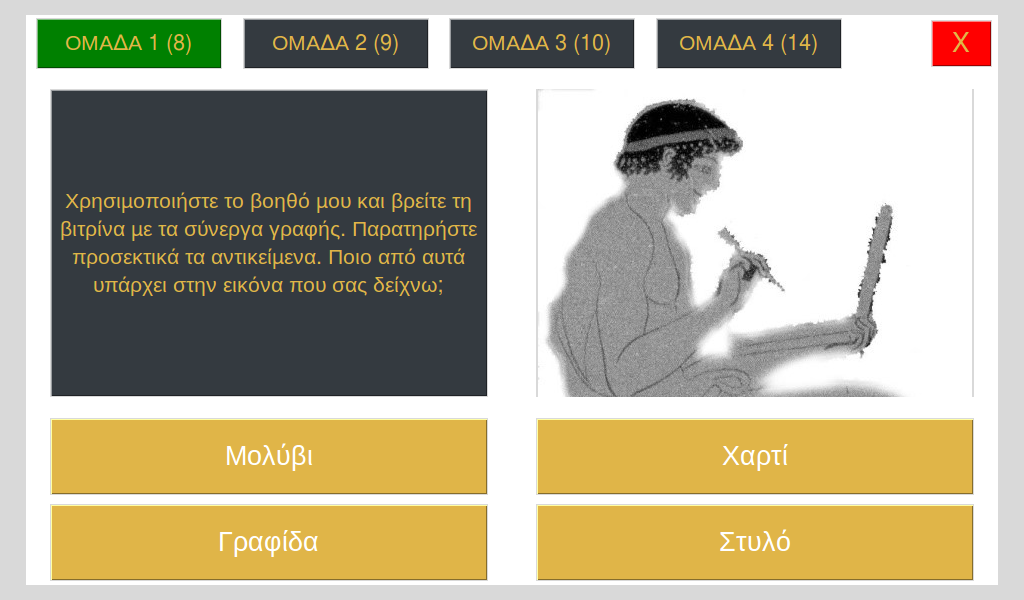
\includegraphics[scale=0.4]{images/cultureid/sc4.png}
  \caption{\small A typical game screen displayed at the robot's mounted
           monitor. The question asks of the pupils to use a handheld RFID
           scanner and point it to the direction of the right artefacts in
           order to provide the correct answer}
  \label{fig:cultureid_sc4}
\end{figure}
\begin{figure}[H]\centering
  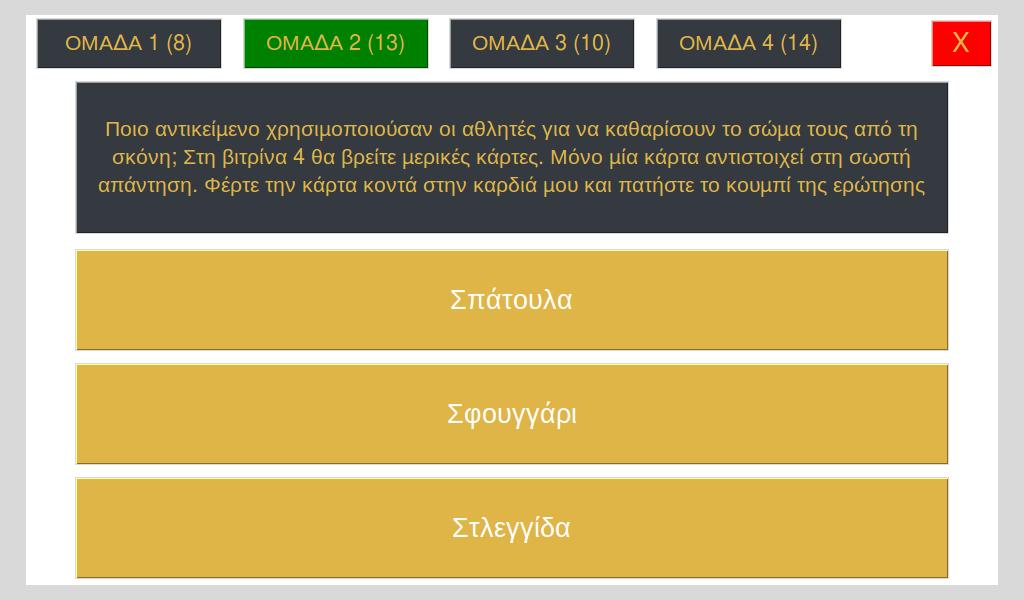
\includegraphics[scale=0.4]{images/cultureid/sc8.png}
  \caption{\small A typical game screen displayed at the robot's mounted
           monitor. The question asks of the pupils to walk around the museum,
           locate RFID tags imprinted with the correct answer, bring it to the
           robot, and scan it using its mounted RFID reader}
  \label{fig:cultureid_sc8}
\end{figure}
\begin{figure}[H]\centering
  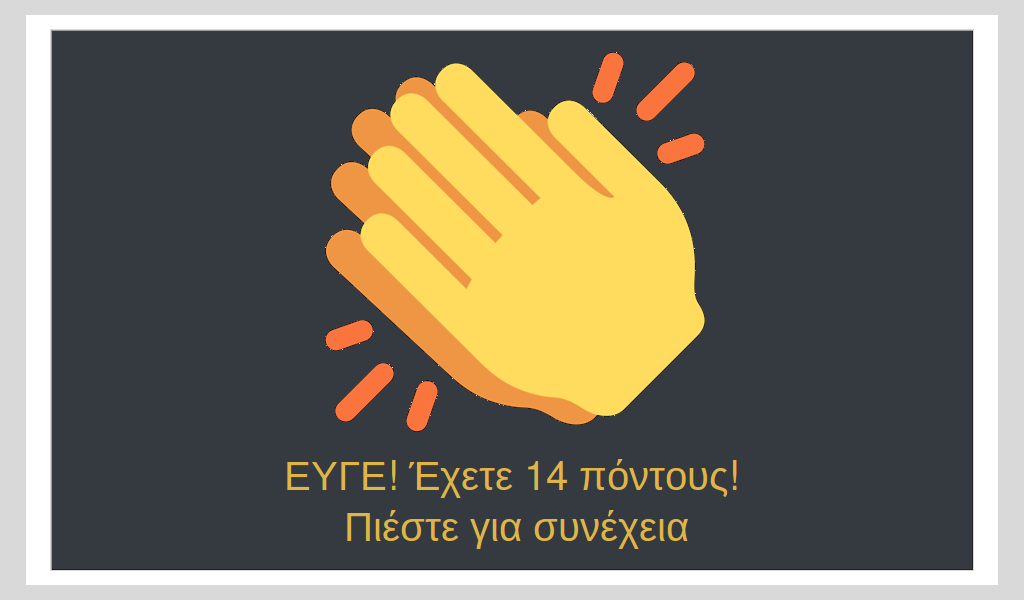
\includegraphics[scale=0.3]{images/cultureid/sc2.png}
  \caption{\small A screen cheering on a team when they provided the correct
           answer}
  \label{fig:cultureid_sc2}
\end{figure}

Images \ref{fig:cultureid_indy_kids_0}-\ref{fig:cultureid_indy_kids_2} show
comments left by students of the 28th public elementary school of Thessaloniki
regarding their experience playing games with the project's social robot.


\begin{figure}[H]\centering
  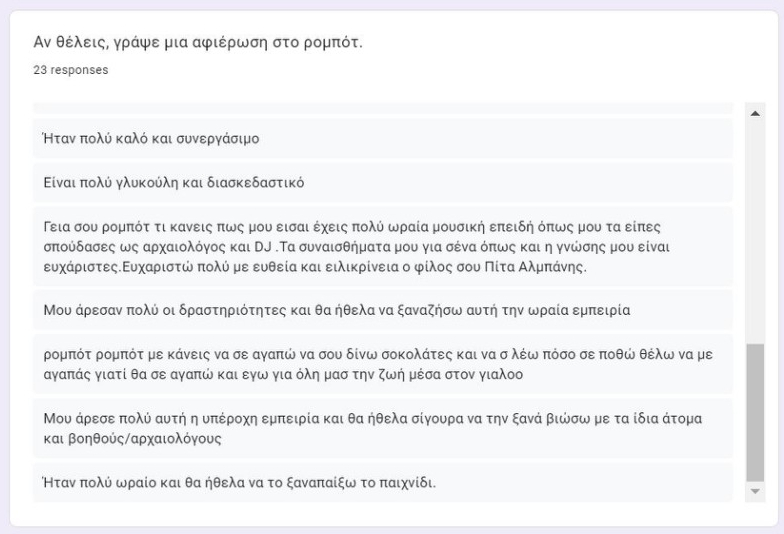
\includegraphics[scale=0.8]{images/cultureid/indy_kids_0.jpg}
  \caption{\small Pupils' feedback on their experience playing games with
           the robot (1/3)}
  \label{fig:cultureid_indy_kids_0}
\end{figure}
\begin{figure}[H]\centering
  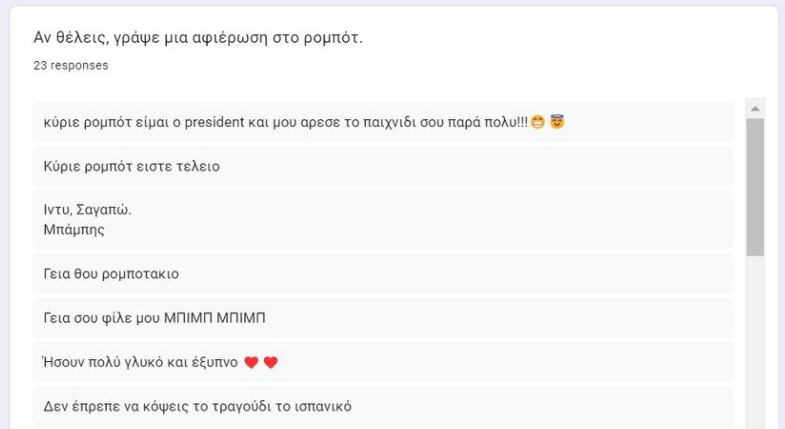
\includegraphics[scale=0.8]{images/cultureid/indy_kids_1.jpg}
  \caption{\small Pupils' feedback on their experience playing games with
           the robot (2/3)}
  \label{fig:cultureid_indy_kids_1}
\end{figure}
\begin{figure}[H]\centering
  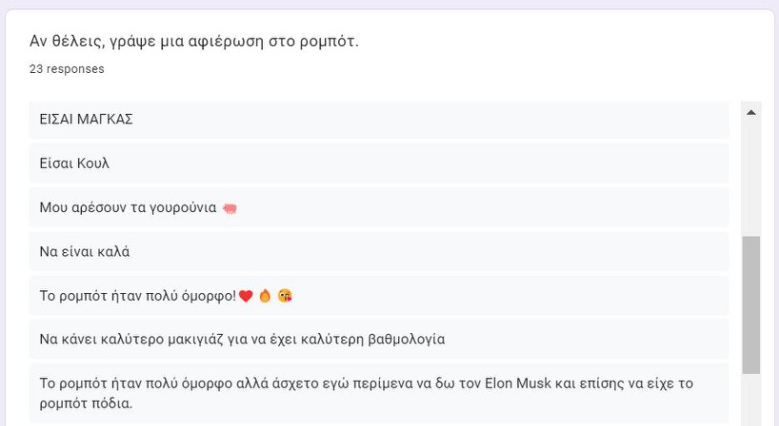
\includegraphics[scale=0.8]{images/cultureid/indy_kids_2.jpg}
  \caption{\small Pupils' feedback on their experience playing games with
           the robot (3/3)}
  \label{fig:cultureid_indy_kids_2}
\end{figure}



\subsubsection{Tour guide}
The second functionality of Indy was acting as a tour guide. The role of the
robot was to sit besides three important artefacts and interact with visitors
when they asked her for further details. In a nutshell, three main datasets
were developed, one pertaining exactly to each artefact, with the expert help
of the Museum's archaeologists. Then rasa was built around these scenarios. The
text-to-speech and speech-to-text was handled by Google. Sound was captured via
a panoramic microphone array, which was specifically chosen with conversation
in mind. \\


\noindent Key project aspects are succinctly portrayed through the following videos:

\begin{itemize}
  \singlespacing
  \item \href{https://www.youtube.com/watch?v=SOA0To077WQ}{CultureID in 80 seconds}
  \item \href{https://www.youtube.com/watch?v=2EvTGNOqTrs}{Games with the Robot in the Museum}
  \item \href{https://www.youtube.com/watch?v=mrTL3Gep7Xk}{Talking with the robot of the Archaeological Museum of Thessaloniki}
  \item \href{https://www.youtube.com/watch?v=i5CUBswHWf0}{Recording of the project's final scientific symposium}
\end{itemize}




\begin{figure}[H]\centering
  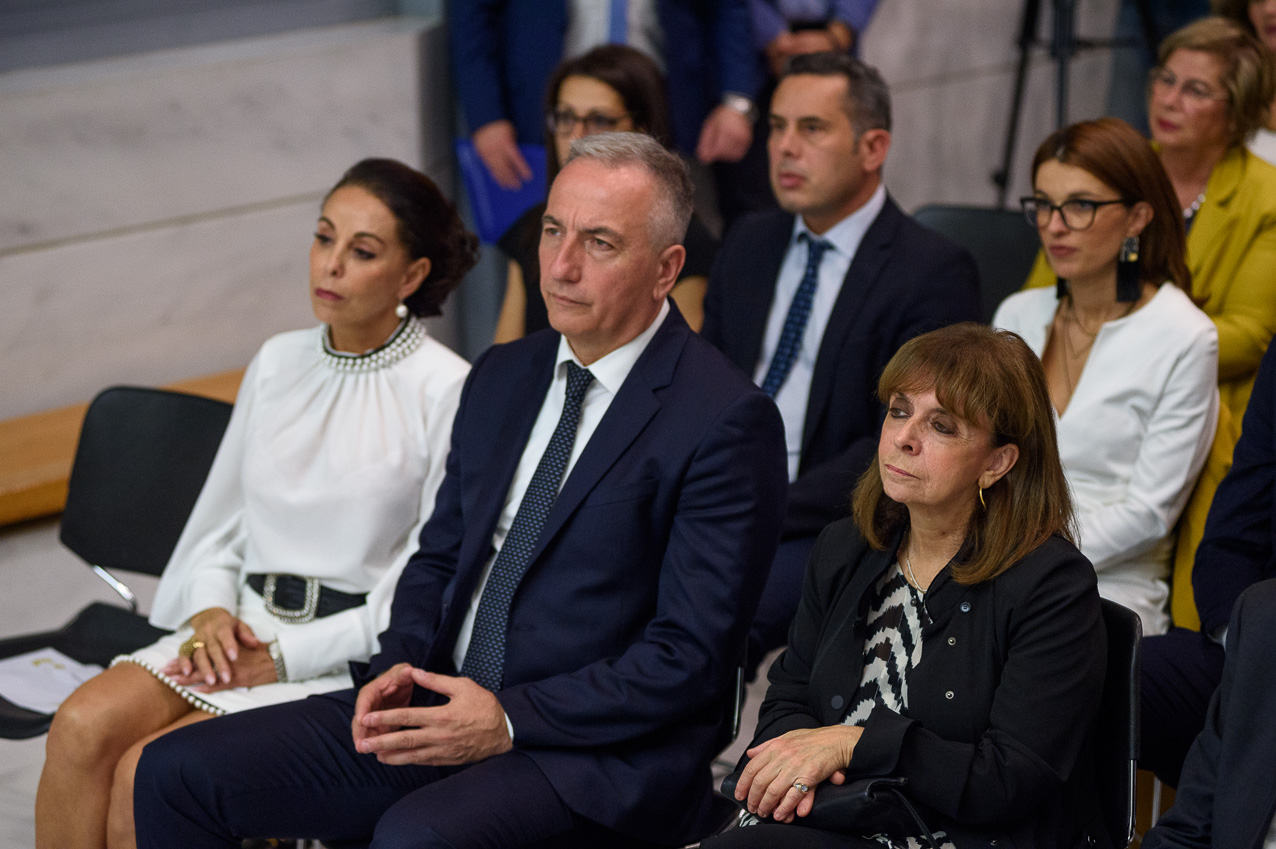
\includegraphics[scale=0.35]{images/cultureid/omg1.jpg}
  \caption{\small From front to back and left to right: the Deputy Head of the
           Region of Thessaloniki, the Deputy Minister for Macedonia and Thrace,
           the President of the Hellenic Republic, Dr Aggeliki Moneda, Dr
           Antonios Dimitriou, and Dr Stavroula Siachalos. The latter three
           belong to CultureID's organisational and administration team.
           Dr Dimitriou was the project's coordinator. The event was the
           celebration of the Archaeological Museum's sixtieth birthday, in
           which CultureID was invited to contribute with its objective and
           results.  Source: \url{https://shorturl.at/tzMT2}}
  \label{fig:cultureid_omg1}
\end{figure}
\begin{figure}[H]\centering
  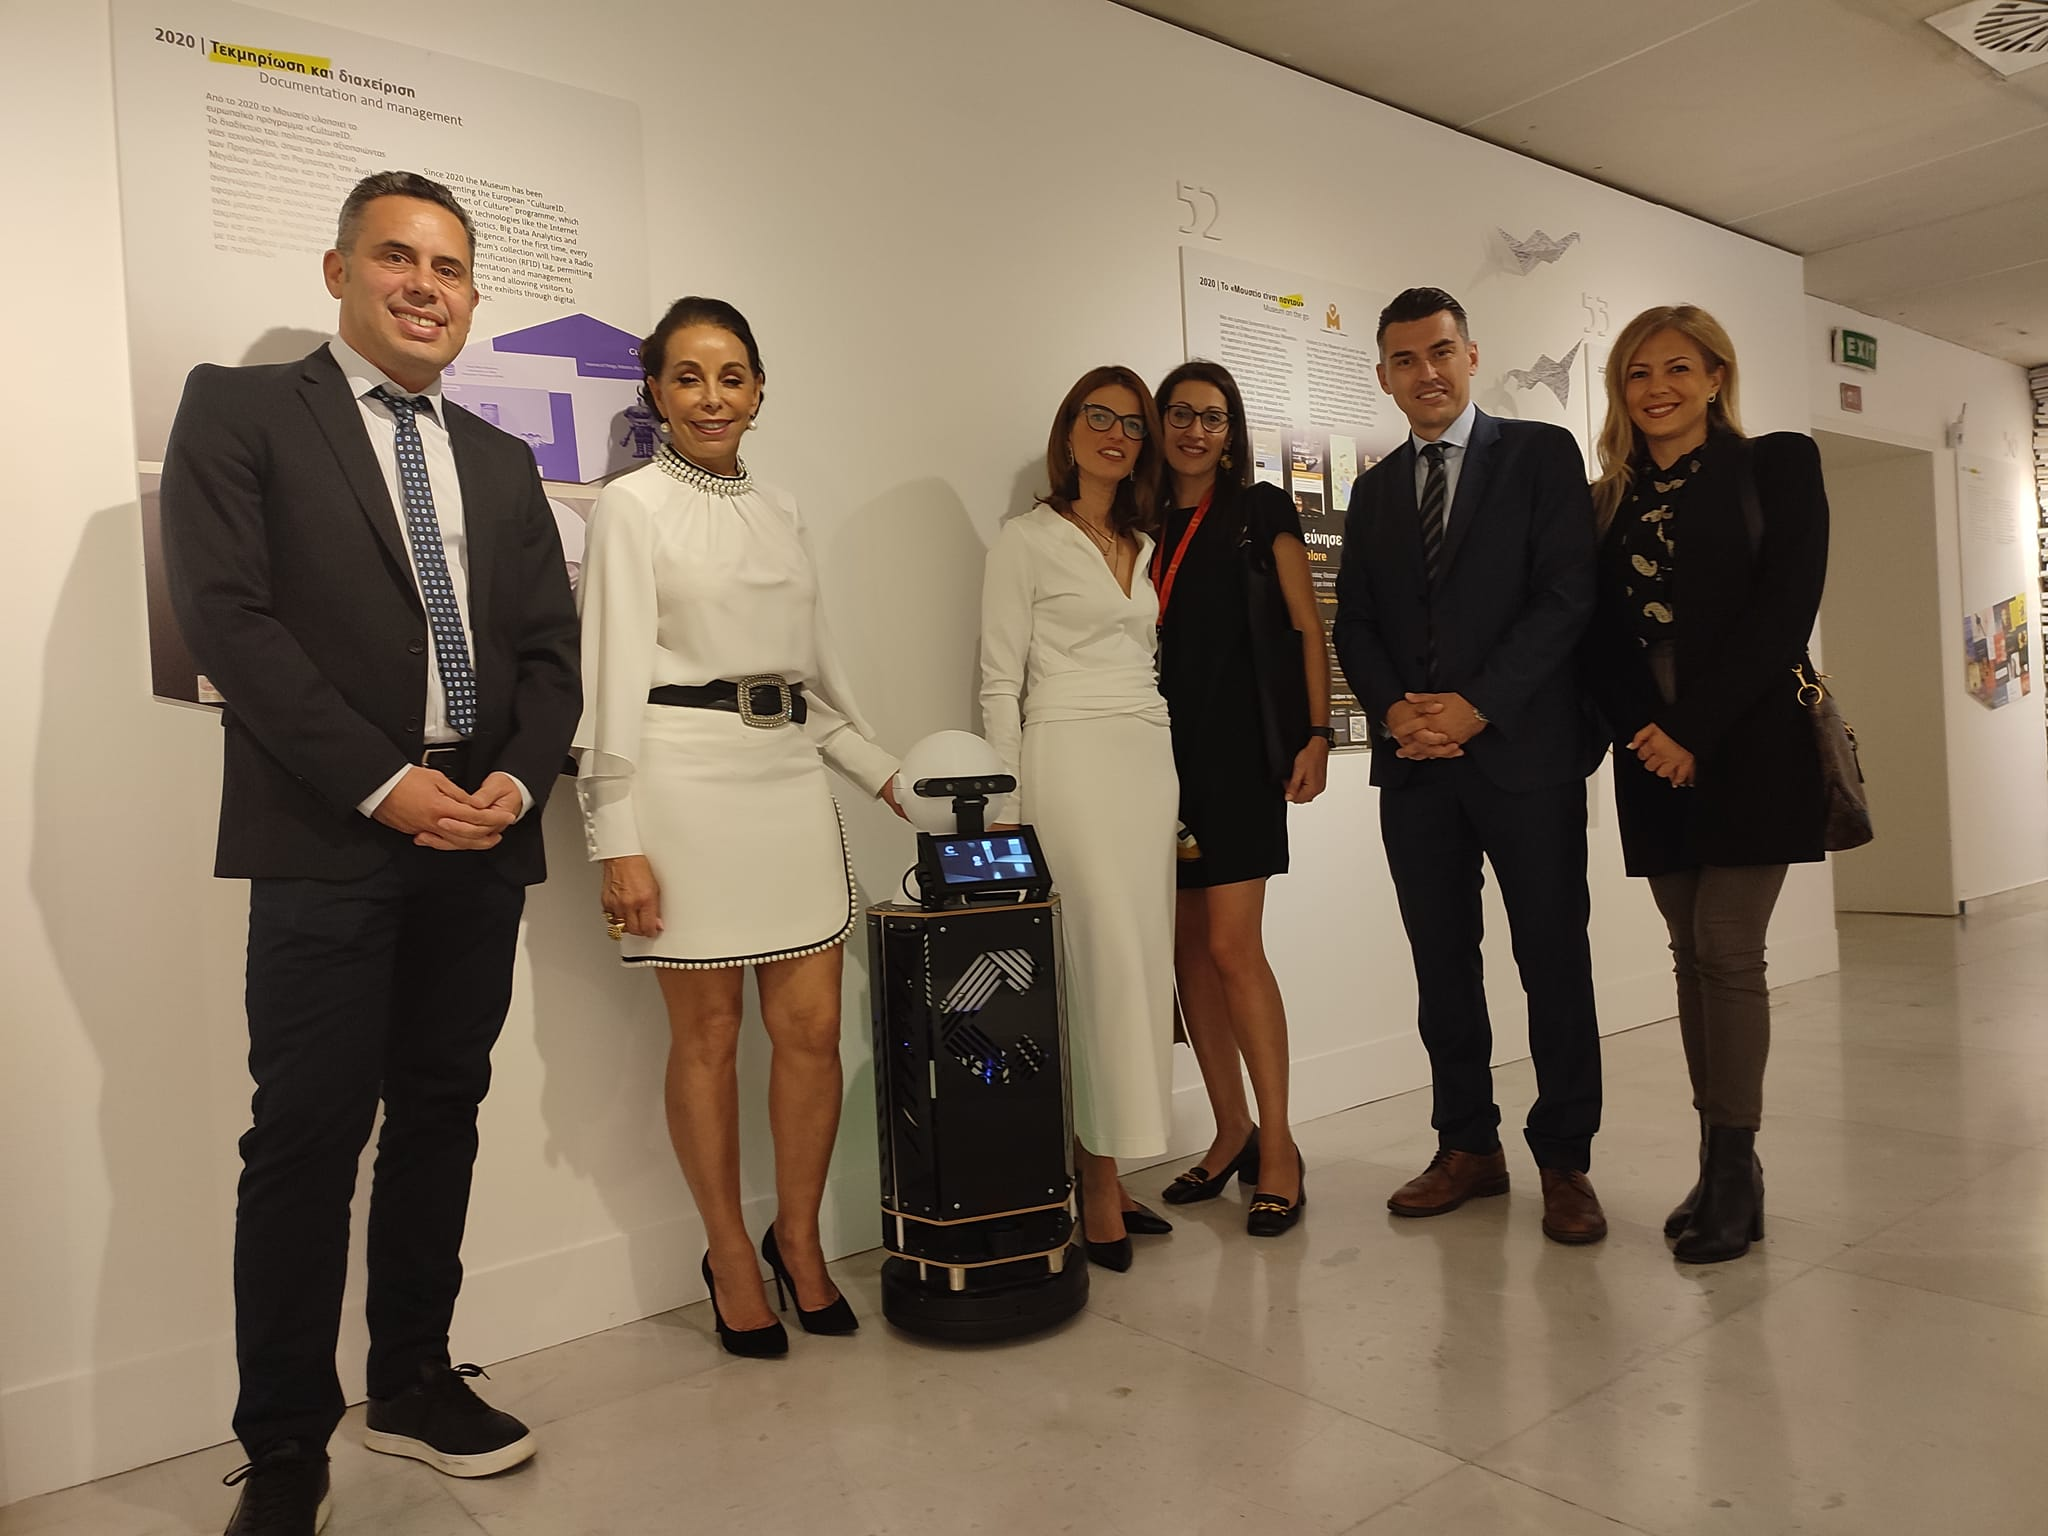
\includegraphics[scale=0.2]{images/cultureid/omg2.jpg}
  \caption{\small From left to right: CultureID's coordinator, Indy, the Deputy
           Head of the Region of Thessaloniki, Dr Stavroula Siachalos, Dr
           Aggeliki Moneda, the Deputy Head of Digital Governance for the
           Region of Central Macedonia, and Ms. Mariana Politou, at the
           celebration of the Archaeological Museum of Thessaloniki's sixtieth
           birthday}
  \label{fig:cultureid_omg2}
\end{figure}
